\documentclass[12pt,a4paper]{article}
\usepackage[legalpaper, portrait, margin=3cm]{geometry}
\usepackage{fancyhdr}
\usepackage{amsmath}
\usepackage{amssymb}
\usepackage{graphicx}
\usepackage{wrapfig}
\usepackage{blindtext}
\usepackage{hyperref}
\usepackage{tikz}

\graphicspath{ {./} }
\hypersetup{
  colorlinks=true,
  linkcolor=blue,
  filecolor=magenta,
  urlcolor=blue,
  citecolor=blue,
  pdftitle={Relatório ASA Projeto 2 2021/2022},
  pdfpagemode=FullScreen,
}

\pagestyle{fancy}
\fancyhf{}
\rhead{Grupo \textbf{al007}}
\lhead{Relatório Projeto 2 ASA 2021/2022 LEIC-A}
\cfoot{Diogo Correia (99211) e Tomás Esteves (99341)}

\renewcommand{\footrulewidth}{0.2pt}

\renewcommand{\labelitemii}{$\circ$}
\renewcommand{\labelitemiii}{$\diamond$}

\begin{document}
  \section{Descrição do Problema e da Solução}

  Pretende-se encontrar, dada uma árvore geneológica e dois nós, os ancestrais comuns mais próximos de ambos os nós.

  Para resolver o \textbf{problema} utilizou-se uma lista de nós.
  Um nó é composto pela identificação dos seus pais, o número de filhos que tem.
  Para otimizar a utilização de memória, apenas é guardado o número de filhos, não quais são, visto que estes não são necessários à resolução do problema.
  Ao decorrer da solução, trabalhamos maioritariamente no grafo transposto, que tem a vantagem de cada nó ter, no máximo, dois arcos.

  O primeiro passo é verificar que o input dado é uma árvore geneológica válida.
  Para tal, é feito o seguinte:
  
  \begin{itemize}
    \setlength{\itemsep}{0pt}
      \item Ao ler o input verifica-se se um nó tem mais de 2 pais. Caso tenha, a árvore é inválida.
      \item Depois de ser lido o input todo, realiza-se uma DFS e no caso de se detetar que existe uma aresta que toca num nó já aberto mais ainda não fechado (\texttt{GREY}), sabe-se que existe um loop, pelo que a árvore é inválida.
  \end{itemize}

  Caso a árvore seja inválida, o programa escreve "\texttt{0}" e termina.

  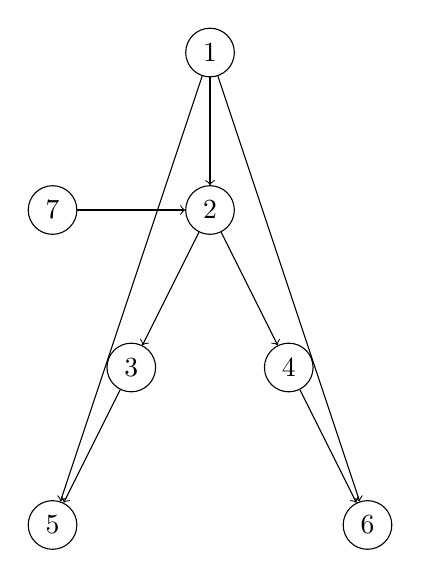
\begin{tikzpicture}[nodes={draw, circle}, ->]
    \node (a1) at (5,7) {1};
    \node (a2) at (5,5) {2};
    \node (a3) at (4,3) {3};
    \node (a4) at (6,3) {4};
    \node (a5) at (3,1) {5};
    \node (a6) at (7,1) {6};
    \node (a7) at (3,5) {7};

    \draw (a1) -> (a2);
    \draw (a2) -> (a3);
    \draw (a2) -> (a4);
    \draw (a3) -> (a5);
    \draw (a4) -> (a6);
    \draw (a1) -> (a5);
    \draw (a1) -> (a6);
    \draw (a7) -> (a2);
  \end{tikzpicture}

  Depois do input ser tratado, são feitas 2 BFS, uma para cada um dos nós para os quais se quer detetar os ancestrais comuns mais próximos.
  Eliminam-se os nós que não pertencem a ambas as BFS.\\
  Explicar pq isto acontece\\
  E finalemente escreve-se por ordem crescente os nós restantes que não têm filhos.\\
 Se nenhum elemento for escrito, o programa escreve "-" e termina.

  \section{Análise Teórica}

  Seja $V$ o número de nós e $E$ o número de arestas.

  \begin{itemize}
    \setlength{\itemsep}{0pt}
    \item No problema começa-se por ler os vértices para os quais se quer detetar os ancestrais comuns mais próximos, assim como o número de nós e o número de arestas, feito em tempo constante, logo $\Theta(1)$:
    \begin{itemize}
      \setlength{\itemsep}{0pt}
      \item De seguida aloca-se dinamicamente memória para lista de nós e é inicializada. Logo, $\Theta(V)$ ou $\Theta(1)$.
      \item Acaba-se por depois tratar da informação relativa aos vértices. Logo, $O(E)$.
    \end{itemize}

   \item É efetuada uma DFS. Logo, $O(V + E)$.

  \item São efetuadas 2 BFS. Logo, $O(V + E)$.

  \item Remover nós que não são comuns a ambas as BFS. Logo, $O(V)$.

  \item Imprimir todos os nós que são ancestrais comuns mais próximos. Logo $\Theta(V)$.
  \end{itemize}
  Logo, no pior caso tem-se $O(V + E)$.\\
  O problema tem complexidade espacial $O(V)$, visto que se utilizou apenas uma lista de tamanho dos números de nós.

  \section{Avaliação Experimental dos Resultados}

  Foi criado instâncias de input com probablidade de criar aresta de 99\% (piot caso), para valores de nós entre 10 e 1000000, qnts por ordem de grandeza (?).\\
  O programa foi executado, pelo menos 100 (?) vezes para cada input, recorrendo ao programa \href{https://github.com/sharkdp/hyperfine}{\textit{hyperfine}}.
    
  \includegraphics[width=1\textwidth]{report.png}
  O gráfico apresentadotem uma escala $V + E$ no eixo dos $xx$ e o tempo em segundos no eixo dos $yy$.\\
  Os dados revelam uma reta (relativamente) linear, comprovando que a complexidade temporal do problema é, num caso geral, $O(V + E)$, tal como concluído na análise teórica.

\end{document}
